\documentclass[11pt]{amsart}
\usepackage[a4paper,margin=1in]{geometry}
\usepackage{amsmath,amssymb,amsthm}
\usepackage[hidelinks]{hyperref}

\newtheorem{theorem}{Theorem}[section]
\newtheorem{lemma}[theorem]{Lemma}
\newtheorem{corollary}[theorem]{Corollary}
\theoremstyle{definition}
\newtheorem{rem}[theorem]{Remark}

\newcommand{\mast}{\operatorname{mast}}

\title[Agreement subtrees of balanced trees]{Agreement subtrees of balanced trees:\\ the exponent exists and lies between $0.243$ and $5/11$}
\author{Vamshi Jandhyala}
\address{London, United Kingdom}
\email{vamshi.jandhyala@gmail.com}

\usepackage{graphicx}
\begin{document}

\begin{abstract}
Let $M(n)$ be the smallest possible size of a maximum agreement subtree of two balanced rooted
binary phylogenetic trees on the same $n=2^m$ leaves. Martin and Thatte conjectured
$M(n)\ge n^{1/2}$. Bordewich, Linz, Owen, St.~John, Semple and Wicke disproved this, showing
$M(n)<c\,n^{1/2}$ for every $c>0$ along a subsequence, and proved $M(n)\ge n^{0.17}$.
A substitution lemma shows that $M$ is submultiplicative, so the exponent
$\beta=\lim \log M(n)/\log n$ exists and equals $\inf_m \log_2 M(2^m)/m$. Their example on
$2048$ leaves then gives $\beta\le 5/11$, that is, $M(n)=O(n^{5/11})$. Optimising the
parameters in their inductive lower bound gives $M(n)\ge n^{0.235}$, and an induction that looks
two levels down one tree and one level down the other gives $M(n)\ge n^{0.243}$. Both steps rest on
inequalities verified by computer in exact and interval arithmetic. Hence
$0.243\le\beta\le 5/11\approx 0.4545$. All of this except the last inequality is also checked in Lean.
\end{abstract}

\maketitle

\section{Introduction}

Maximum agreement subtrees measure how much two phylogenetic trees on the same species have in
common. The extremal question asks how small the largest common restriction can be. For
unrooted binary trees the answer is $\Theta(\log n)$ \cite{Markin}, after earlier bounds by
Steel and Sz\'ekely \cite{SS} and by Martin and Thatte \cite{MT}. For rooted trees without a
shape constraint the question is trivial, since a caterpillar and its reverse agree on only
two leaves. Constraining the shape changes the picture. When both trees are \emph{balanced},
Martin and Thatte proved a polynomial lower bound $n^{\beta_0}$ with $\beta_0\approx 0.149$ and
conjectured that $n^{1/2}$ is the truth \cite[Conjecture~20]{MT}.

Bordewich, Linz, Owen, St.~John, Semple and Wicke \cite{BLOSSW} gave a family of counterexamples.
For every $k\ge1$ they construct balanced trees on $2^{2^{k+1}-k-2}$ leaves whose maximum
agreement subtrees have $2^{2^k-k}$ leaves, which is below $c\,n^{1/2}$ once $k$ is large. They
also raised the lower bound to $n^{0.17}$. In their family the ratio of the agreement size to $n^{1/2}$ tends to zero
only like $(\log n)^{-1/2}$, so it leaves open whether the true growth rate is $n^{1/2-o(1)}$.

For a small case, the balanced trees $((1,2),(3,4))$ and $((1,3),(2,4))$ agree on no three leaves
(Figure~\ref{fig:subst}(a)), so $M(4)=2=4^{1/2}$; for $k=3$ the construction of \cite{BLOSSW} gives
two balanced trees on $2048$ leaves that agree on at most $32$, against $2048^{1/2}\approx45$.
This note settles that point and narrows the range for the exponent from both sides.

\begin{theorem}\label{thm:main}
Let $M(n)$ denote the minimum of $\mast(S,T)$ over all pairs of balanced rooted binary
phylogenetic trees $S,T$ on a common set of $n=2^m$ labels.
\begin{enumerate}
\item The limit $\beta=\lim_{m\to\infty}\log_2 M(2^m)/m$ exists and equals
  $\inf_{m\ge1}\log_2 M(2^m)/m$.
\item $M(n)\le 2^{10}\,n^{5/11}$ for every $n=2^m$. In particular $\beta\le 5/11$.
\item $M(n)\ge n^{0.243}$ for every $n=2^m$. In particular $\beta\ge 0.243$.
\end{enumerate}
\end{theorem}

Part~(1) rests on a substitution lemma (Lemma~\ref{lem:subst}), which is elementary but which we
have not found in the literature on this problem. Its useful consequence is that any single pair of balanced trees
with a small agreement subtree yields a bound for all $n$. Part~(2) applies it to the $k=3$
example of \cite{BLOSSW}. Part~(3) keeps the induction of \cite[Theorem~1.3]{BLOSSW} but
replaces its case analysis by an exact inequality in four variables, checked in interval
arithmetic (Lemma~\ref{lem:cert}), which gives $n^{0.235}$. Looking two levels down one tree and one
level down the other turns this into an inequality in eight variables between finitely many concave
functions, which a certified simplicial subdivision verifies (Lemma~\ref{lem:cert2}); this gives
$n^{0.243}$.

For comparison, two independent uniformly random leaf-labelled binary trees have a maximum
agreement subtree of order at least $n^{0.366}$ \cite{Aldous}, improved to $n^{0.4464}$
\cite{Khezeli}, and typically at most $n^{1/2-\varepsilon}$ \cite{BS}. For two balanced trees
with independent uniform labellings the expected size is $\Theta(n^{1/2})$ \cite{MS}.
Part~(2) therefore shows that suitably chosen balanced trees agree polynomially less than
random labellings of the same shapes.

\section{Preliminaries}

We follow the terminology of \cite{BLOSSW}. A rooted binary phylogenetic $X$-tree is a rooted
binary tree whose leaves are bijectively labelled by $X$. For $Y\subseteq X$ the restriction
$T|Y$ is obtained from the minimal subtree connecting $Y$ by suppressing non-root vertices of
degree two. For trees $S$ and $T$ with label sets $X$ and $X'$, a set $Y\subseteq X\cap X'$ is an
\emph{agreement set} if $S|Y\cong T|Y$ as leaf-labelled trees, and $\mast(S,T)$ is the largest
size of an agreement set. A rooted binary tree is \emph{balanced} if it has $2^m$ leaves, all at
depth $m$. If $S_L,S_R$ and $T_L,T_R$ are the maximal pendant subtrees of $S$ and $T$, then
\begin{equation}\label{eq:rec}
\begin{aligned}
\mast(S,T)=\max\{&\mast(S_L,T_L)+\mast(S_R,T_R),\ \mast(S_L,T_R)+\mast(S_R,T_L),\\
&\mast(S,T_L),\ \mast(S,T_R),\ \mast(S_L,T),\ \mast(S_R,T)\}.
\end{aligned}
\end{equation}
In words, a largest agreement set either meets both halves of both trees, matching the halves in one of the two possible ways, or lies inside one half of one of the trees.

For example, the balanced trees $S=((1,2),(3,4))$ and $T=((1,3),(2,4))$ of Figure~\ref{fig:subst}(a) agree on no three leaves: any three labels contain exactly one cherry of $S$ and exactly one cherry of $T$, and the cherries $\{1,2\},\{3,4\}$ of $S$ never coincide with the cherries $\{1,3\},\{2,4\}$ of $T$. So $M(4)=2=4^{1/2}$.

\begin{figure}[ht]
\centering
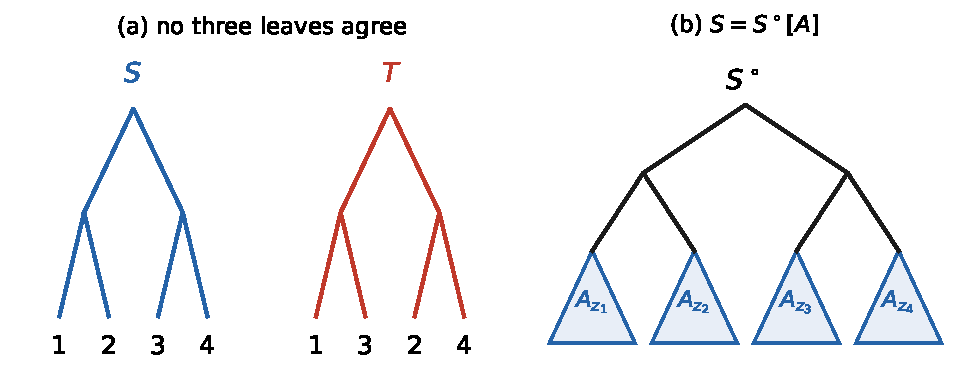
\includegraphics[width=0.74\textwidth]{fig_subst.pdf}
\caption{(a) Two balanced trees on four leaves whose largest agreement subtree has two leaves. (b) The substitution $S^\circ[A]$ of Section~\ref{sec:subst}: each leaf $z$ of $S^\circ$ becomes the root of a tree $A_z$. An agreement set of $S^\circ[A]$ and $T^\circ[B]$ can use at most $\mast(S^\circ,T^\circ)$ of the blocks, and at most $\mast(A_z,B_z)$ leaves inside each.}
\label{fig:subst}
\end{figure}

A \emph{cluster} of a rooted tree is the set of leaves below some vertex. If $C$ is a cluster
of $S$ and $Y$ meets $C$ in exactly one leaf $y$, then for any $c\in C$ the tree $S|Y$ is
obtained from $S|((Y\setminus C)\cup\{c\})$ by renaming $c$ as $y$.

\section{Substitution and the existence of the exponent}\label{sec:subst}

Let $S^\circ$ and $T^\circ$ be rooted binary phylogenetic trees on a label set $Z$. For each
$z\in Z$ let $A_z$ and $B_z$ be rooted binary phylogenetic trees on a label set $\Lambda_z$,
where the sets $\Lambda_z$ are pairwise disjoint. Write $S=S^\circ[A]$ for the tree obtained from
$S^\circ$ by identifying each leaf $z$ with the root of $A_z$, and define $T=T^\circ[B]$ in the
same way (Figure~\ref{fig:subst}(b)). Each $\Lambda_z$ is then a cluster of both $S$ and $T$.

\begin{lemma}[Substitution]\label{lem:subst}
With this notation,
\[
\mast(S,T)\le \mast(S^\circ,T^\circ)\cdot\max_{z\in Z}\mast(A_z,B_z).
\]
\end{lemma}

\begin{proof}
Let $Y$ be an agreement set for $S$ and $T$, and let $Z_Y=\{z: Y\cap\Lambda_z\ne\emptyset\}$.
Choose one label $y_z\in Y\cap\Lambda_z$ for each $z\in Z_Y$ and put $Y'=\{y_z:z\in Z_Y\}$.
Since each $\Lambda_z$ is a cluster of $S$ met by $Y'$ in exactly one leaf, $S|Y'$ is
$S^\circ|Z_Y$ with $z$ renamed $y_z$, and likewise $T|Y'$ is $T^\circ|Z_Y$ renamed. Now
$S|Y'=(S|Y)|Y'\cong(T|Y)|Y'=T|Y'$, so $Z_Y$ is an agreement set of $S^\circ$ and $T^\circ$ and
$|Z_Y|\le\mast(S^\circ,T^\circ)$. For each $z$, the restrictions of $S$ and $T$ to
$Y\cap\Lambda_z$ are $A_z|(Y\cap\Lambda_z)$ and $B_z|(Y\cap\Lambda_z)$, and they agree, so
$|Y\cap\Lambda_z|\le\mast(A_z,B_z)$. Summing over $z\in Z_Y$ gives the bound.
\end{proof}

\begin{corollary}\label{cor:submult}
For all $h,k\ge0$, $M(2^{h+k})\le M(2^h)\,M(2^k)$.
\end{corollary}

\begin{proof}
Take $S^\circ,T^\circ$ balanced of height $h$ with $\mast(S^\circ,T^\circ)=M(2^h)$, and for every
$z$ take $(A_z,B_z)$ to be a copy, relabelled onto $\Lambda_z$, of a balanced pair of height $k$
attaining $M(2^k)$. Then $S$ and $T$ are balanced of height $h+k$ on the same $2^{h+k}$
labels, and Lemma~\ref{lem:subst} applies.
\end{proof}

For example, substituting the pair of Figure~\ref{fig:subst}(a) into itself gives balanced trees on $16$ leaves whose largest agreement subtree has $4$ leaves, so $M(16)\le4$.

\begin{proof}[Proof of Theorem~\ref{thm:main}(1)]
The sequence $a_m=\log_2 M(2^m)$ is nonnegative and, by Corollary~\ref{cor:submult},
subadditive. Fekete's lemma \cite{Fekete} gives $\lim a_m/m=\inf a_m/m$.
\end{proof}

\section{The upper bound}

\begin{proof}[Proof of Theorem~\ref{thm:main}(2)]
Taking $k=3$ in \cite[Theorem~4.6]{BLOSSW} gives balanced trees on $2^{11}=2048$ leaves with
maximum agreement subtrees of size $2^5=32$, so $M(2^{11})\le 2^5$. (The trees are listed in
Newick format in \cite[Appendix~A]{BLOSSW}; we recomputed the value $32$ for exactly these trees,
see Section~\ref{sec:verify}.) Write $m=11j+r$ with $0\le r\le 10$. Corollary~\ref{cor:submult} and
the trivial bound $M(2^r)\le 2^r$ give
\[
M(2^m)\le M(2^{11})^j\,M(2^r)\le 2^{5j}\,2^r\le 2^{5m/11}\,2^{10}.\qedhere
\]
\end{proof}

Iterating the substitution gives explicit examples. For instance, substituting the $2048$-leaf
pair into itself produces balanced trees on $2^{22}$ leaves with no agreement subtree larger
than $2^{10}$, whereas $n^{1/2}=2^{11}$.

\begin{rem}\label{rem:family}
The construction of \cite{BLOSSW} arranges $p=2^{h_1}$ pendant subtrees of height $h_2$ in each
tree as a grid, and fills each of the $p^2$ cells with a caterpillar that is reversed in the
other tree; this uses caterpillars of length at most $h_2+1$, so $p(h_2+1)\ge 2^{h_2}$, and
gives agreement $2p$ on $p\,2^{h_2}$ leaves. Combined with substitution, one such pair yields
the exponent $(1+h_1)/(h_1+h_2)$. Over all $(h_1,h_2)$ allowed by the length constraint this is
minimised at $(h_1,h_2)=(4,7)$, the case $k=3$, with value $5/11$. Going below $5/11$ therefore
needs a different gadget, not a different choice of parameters.
\end{rem}

\section{The lower bound}

For balanced trees $S$ and $T$ of heights $h_1$ and $h_2$ whose label sets share exactly $t\ge1$
labels, let $g(h_1,h_2,t)$ be the minimum possible value of $\mast(S,T)$. Following
\cite[Theorem~1.3]{BLOSSW}, an estimate of the form
\begin{equation}\label{eq:ansatz}
g(h_1,h_2,t)\ \ge\ t^{a}\,2^{-c(h_1+h_2)}
\end{equation}
gives $M(n)\ge n^{a-2c}$ on putting $h_1=h_2=\log_2 n$ and $t=n$. The paper \cite{BLOSSW} takes
$(a,c)=(0.22,0.025)$, giving the exponent $0.17$. The induction closes for any $(a,c)$
satisfying the inequality below. For $x=(x_1,x_2,x_3,x_4)$ with nonnegative entries set
\[
\Phi_{a,c}(x)=\max\Bigl\{4^c(x_1^a+x_4^a),\ 4^c(x_2^a+x_3^a),\ 2^c(x_1+x_2)^a,\ 2^c(x_3+x_4)^a,\
2^c(x_1+x_3)^a,\ 2^c(x_2+x_4)^a\Bigr\},
\]
with the convention $0^a=0$, and let $\Delta=\{x\ge0: x_1+x_2+x_3+x_4=1\}$.

In the induction, $x_1,\dots,x_4$ are the fractions of the shared labels lying in the four overlap cells $S_p\cap T_q$, and the six terms of $\Phi_{a,c}$ are the six cases of~\eqref{eq:rec}: the two diagonals, where both trees lose a level, and the two rows and two columns, where one tree does (Figure~\ref{fig:grid}). The inequality says that whichever way the shared labels are spread over the cells, at least one case keeps enough of them.

\begin{figure}[ht]
\centering
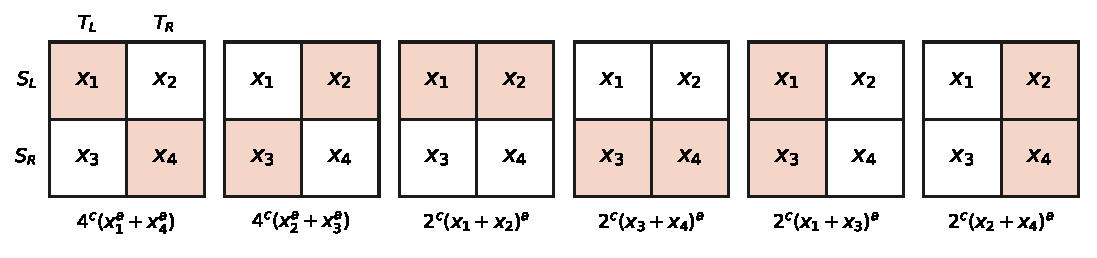
\includegraphics[width=0.9\textwidth]{fig_grid.pdf}
\caption{The six terms of $\Phi_{a,c}$ as the six cases of recurrence~\eqref{eq:rec}, read on the table of overlaps $x_1,\dots,x_4$ between the halves of $S$ (rows) and of $T$ (columns).}
\label{fig:grid}
\end{figure}

\begin{lemma}[computer-assisted]\label{lem:cert}
For $a=2/5$ and $c=33/400$, $\Phi_{a,c}(x)\ge 1$ for every $x\in\Delta$.
\end{lemma}

\begin{proof}
Each of the six expressions in $\Phi_{a,c}$ is nondecreasing in each coordinate. Parametrise
$\Delta$ by $(x_1,x_2,x_3)$ with $x_4=1-x_1-x_2-x_3$. On a box
$\prod_{i\le3}[l_i,u_i]$, every point of $\Delta$ satisfies $x_i\ge l_i$ for $i\le 3$ and
$x_4\ge \max(0,1-u_1-u_2-u_3)$, so $\Phi_{a,c}$ is bounded below on the box by its value at
$(l_1,l_2,l_3,\max(0,1-u_1-u_2-u_3))$. Starting from $[0,1]^3$, a box is discarded if
$l_1+l_2+l_3>1$, accepted if this lower bound is at least $1$, and otherwise bisected along its
longest side. Box corners are exact dyadic rationals, $a$ and $c$ are the exact rationals above, and
each expression is evaluated in interval arithmetic at $40$ significant digits; a box is accepted only
when the lower endpoint of some expression's interval is at least $1$. The procedure terminates after
examining $4373$ boxes, the smallest of side $2^{-12}$, with every box accepted or discarded.
\end{proof}

\begin{proof}[Proof that $M(n)\ge n^{0.235}$]
We prove \eqref{eq:ansatz} with $(a,c)=(2/5,33/400)$ by induction on $h_1+h_2$. If $h_1=0$ or
$h_2=0$, one tree is a single leaf, so $t=1$ and $g=1\ge 2^{-c(h_1+h_2)}$. Otherwise let
$S_L,S_R,T_L,T_R$ be the maximal pendant subtrees, and let $t\,x_1$, $t\,x_2$, $t\,x_3$,
$t\,x_4$ be the numbers of shared labels in $S_L\cap T_L$, $S_L\cap T_R$, $S_R\cap T_L$ and
$S_R\cap T_R$, so that $x\in\Delta$. Apply the induction hypothesis to each term of
\eqref{eq:rec}; a term whose two trees share no labels is $0$, which matches $0^a=0$. For
example
\[
\mast(S_L,T_L)+\mast(S_R,T_R)\ \ge\ \bigl((tx_1)^a+(tx_4)^a\bigr)2^{-c(h_1+h_2-2)}
= t^a2^{-c(h_1+h_2)}\cdot 4^c(x_1^a+x_4^a),
\]
and $\mast(S_L,T)\ge (t(x_1+x_2))^a\,2^{-c(h_1+h_2-1)}=t^a2^{-c(h_1+h_2)}\cdot2^c(x_1+x_2)^a$. The
six terms give $\mast(S,T)\ge t^a2^{-c(h_1+h_2)}\,\Phi_{a,c}(x)$, and Lemma~\ref{lem:cert}
completes the induction, and gives $M(n)\ge n^{a-2c}$ with $a-2c=2/5-33/200=0.235$.
\end{proof}

\begin{rem}
Numerical optimisation over $(a,c)$ indicates that this induction cannot give an exponent
larger than about $0.2354$, attained near $a=0.40$. The binding configurations lie near
$x\approx(0.73,0.13,0.13,0)$: one of the four overlap cells holds most of the shared labels
and the rest is split evenly across the two off-diagonal cells. Further progress on the lower bound needs more than a
one-level induction.
\end{rem}

\subsection*{A two-level induction}
Keep the ansatz \eqref{eq:ansatz}, but when $h_1\ge2$ and $h_2\ge1$ expand $S$ two levels and $T$ one
level. Index the four subtrees of $S$ at depth two by $p\in\{00,01,10,11\}$ and the two subtrees of
$T$ at depth one by $q\in\{0,1\}$, and let $t\,y_{pq}$ be the number of shared labels in $S_p\cap T_q$,
so that $y$ lies in the simplex $\Delta_8$ of dimension seven. For a vertex $u$ of $S$ at depth at most two and
a vertex $v$ of $T$ at depth at most one, write $L_{uv}(y)$ for the sum of $y_{pq}$ over the leaves $p$
below $u$ and $q$ below $v$, so that $t\,L_{uv}(y)$ labels are shared by $S_u$ and $T_v$.

Applying \eqref{eq:rec} to the pair $(S,T)$ and then again to pairs of subtrees, as long as both stay
within the expanded levels, and stopping at pairs $(S_u,T_v)$ other than $(S,T)$ itself, bounds
$\mast(S,T)$ below by a sum of terms $\mast(S_u,T_v)$ over disjoint pairs. Call each such choice a
\emph{strategy}; there are $42$. Every stopped pair has smaller total height, so the induction
hypothesis gives $\mast(S_u,T_v)\ge (t\,L_{uv}(y))^a\,2^{-c(h_1+h_2-|u|-|v|)}$, where $|u|,|v|$ are the
depths. Hence
\[
\mast(S,T)\ \ge\ t^a 2^{-c(h_1+h_2)}\max_j \varphi_j(y),\qquad
\varphi_j(y)=\sum_{(u,v)\in j} 2^{c(|u|+|v|)}\,L_{uv}(y)^a .
\]
Each $\varphi_j$ is a nonnegative combination of concave functions of $y$, so it is concave on
$\Delta_8$.

\begin{lemma}[computer-assisted]\label{lem:cert2}
For $a=2/5$ and $c=157/2000$, $\max_j\varphi_j(y)\ge1$ for every $y\in\Delta_8$.
\end{lemma}

\begin{proof}
Subdivide $\Delta_8$ by repeatedly bisecting the longest edge of a simplex. A simplex is certified if
some $\varphi_j$, or some combination $\sum_j\lambda_j\varphi_j$ with $\lambda_j\ge0$ and
$\sum_j\lambda_j\le1$, is at least $1$ at all of its vertices. Such a combination is concave and at most
$\max_j\varphi_j$ (as each $\varphi_j\ge0$), and a concave function attains its minimum over a simplex
at a vertex, so the lemma holds on a certified simplex. The subdivision of $\Delta_8$ into $1{,}418{,}968$
certified simplices, of maximum depth $47$, is found by a floating-point search and each certificate is
then checked rigorously. The vertices are dyadic, and are handled as exact integers over $2^{52}$, so
every value $L_{uv}$ is exact. For each power $x^{2/5}$ and each weight $2^{c(|u|+|v|)}$, a floating-point
lower bound $r$ is used only after checking $r^5\le x^2$, respectively
$r^{2000}\le 2^{157(|u|+|v|)}$, in exact integer arithmetic. The final sums, of at most a few dozen
terms, are required to exceed $1+2^{-40}$, which is more than their worst-case rounding error, and the
weights $\lambda_j$ are checked to sum to at most $1$ in exact rational arithmetic. Of the simplices,
$1{,}042{,}855$ are certified by a combination and the rest by a single strategy.
\end{proof}

\begin{proof}[Proof of Theorem~\ref{thm:main}(3)]
We prove \eqref{eq:ansatz} with $(a,c)=(2/5,157/2000)$ by induction on $h_1+h_2$. By symmetry of
$\mast$ we may assume $h_1\ge h_2$. If $h_1\le1$ or $h_2=0$, one tree has at most two leaves, so
$t\le2$; any set of at most two shared labels is an agreement set, so
$\mast(S,T)=t\ge t^a\ge t^a2^{-c(h_1+h_2)}$. Otherwise $h_1\ge2$ and $h_2\ge1$, and the display above
together with Lemma~\ref{lem:cert2} completes the induction. Putting $h_1=h_2=m$ and $t=n=2^m$ gives
$M(n)\ge n^{a-2c}$ with $a-2c=2/5-157/1000=243/1000$.
\end{proof}

\begin{rem}
The same certifier finds a point where the inequality fails for $c=19/250$, so with $a=2/5$ this
induction gives no exponent above about $0.248$. At $a=2/5$, local search from that point places
the threshold near $c\approx0.0776$, an exponent of about $0.245$.
\end{rem}

\section{Verification}\label{sec:verify}

All claims involving computation were checked with short scripts, available with the Lean files at
\url{https://github.com/jvvk/mathematics}.
\begin{itemize}
\item An exact dynamic program for $\mast$ of two balanced trees, based on \eqref{eq:rec} and
  restricted to pairs of subtrees with overlapping label sets, agrees with brute-force
  enumeration on $300$ random pairs with at most $16$ leaves.
\item Parsing the two trees printed in \cite[Appendix~A]{BLOSSW} confirms that both are balanced of
  height $11$ on the labels $1,\dots,2048$, and the program gives $\mast(S,T)=32$ for them.
\item Rebuilding the construction of \cite[Theorem~4.6]{BLOSSW} with $k=3$ gives agreement
  exactly $32$ on $2048$ leaves. Substituted pairs give exactly the product bound, for example
  agreement $128$ on $2^{15}$ leaves from the $k=2$ and $k=3$ pairs. When the caterpillars are
  not reversed the same program reports $128$ on $2048$ leaves, so it does detect a broken
  construction.
\item The certificate of Lemma~\ref{lem:cert} succeeds for $(a,c)=(2/5,33/400)$ and fails, as it
  should, for $(2/5,2/25)$, which lies below the numerical threshold.
\item The certificate of Lemma~\ref{lem:cert2} succeeds for $(a,c)=(2/5,157/2000)$ in $582$ seconds and
  finds a violating vertex, as it should, for $(2/5,19/250)$. Every simplex accepted by the
  floating-point search also passed the rigorous check. The exact lower bounds for $x^{2/5}$ were
  compared with $60$-digit values at $20{,}000$ random arguments and never exceeded them, and a
  deliberately inflated bound fails the exact test.
\item The $42$ strategies are generated mechanically from \eqref{eq:rec}. With one level on each side
  the same generator and the simplicial certifier reproduce Lemma~\ref{lem:cert}, in $331$ simplices.
\end{itemize}

\section{Formal verification}\label{sec:lean}

Everything above except Lemma~\ref{lem:cert2} is checked in Lean~4 with Mathlib
\cite{mathlib}, using only the standard axioms. The formal development follows the text.
\begin{itemize}
\item Agreement is defined through displayed triples, and a separate theorem shows that this is the
  usual definition: $Y$ is an agreement set exactly when $S|Y\cong T|Y$, because a rooted binary
  phylogenetic tree is determined by its triples.
\item Lemma~\ref{lem:subst}, Corollary~\ref{cor:submult} and Theorem~\ref{thm:main}(1) (Fekete's
  lemma is in Mathlib).
\item Theorem~\ref{thm:main}(2), with $M(2^{11})\le 2^5$ proved, not quoted: Lemma~4.5 of
  \cite{BLOSSW} is formalised with their proof, and applied to an explicit pair of balanced trees on
  $2048$ leaves built as in their Theorem~4.6 from sixteen $8$-caterpillars packing a tree of height $7$
  (found by the recursion of their Lemma~4.3).
\item The one-level induction and Lemma~\ref{lem:cert}, hence $M(n)\ge n^{0.235}$. Lean checks a second,
  integer certificate for Lemma~\ref{lem:cert}: $1638$ boxes on the grid of step $1/N$, $N=2^{16}$.
  A lower bound $r/2^{24}$ for $x^{2/5}$ at a grid value $x=S/N$ is certified by the integer inequality
  $r^5N^2\le S^2 2^{120}$, and lower bounds for $2^c$ and $4^c$ by their $400$th and $200$th powers. The boxes are found by a short script; Lean only checks them.
\item The two-level induction with the $42$ strategies, which are generated mechanically and compared
  with those of the certifier. Lean proves $M(n)\ge n^{0.243}$ from the inequality of
  Lemma~\ref{lem:cert2}, which enters as a hypothesis.
\end{itemize}
The certificate of Lemma~\ref{lem:cert2}, with over a million simplices, is checked in exact arithmetic by
the script of Section~\ref{sec:verify} and not in Lean. Fourteen mutations of the formal development
(a wrong constant, a caterpillar left unreversed, an inflated bound) each make it fail to compile. The Lean files
and scripts are at \url{https://github.com/jvvk/mathematics}.

\section{Open questions}

The exponent $\beta$ now lies in $[0.243,\,5/11]$. By Theorem~\ref{thm:main}(1), any pair of
balanced trees on $2^m$ leaves with agreement less than $2^{5m/11}$ improves the upper bound.
Local search over labellings found no such pair with at most $64$ leaves.
A natural way to shorten the caterpillars in Remark~\ref{rem:family} would be to use pairs of
lower height in which no triple is displayed by both trees. Exhaustive enumeration shows that
for $5\le r\le 7$ every such pair on $r$ leaves contains a tree of height $r-1$, so for these
sizes the caterpillar is already optimal. Whether $\beta$ is close to $5/11$ or substantially smaller is open.

\section*{Acknowledgements}
The author used an AI assistant, Claude (Anthropic; Claude Opus~5.5 for the formalisation). It
found the substitution argument and the two-level induction, wrote the certifiers and the other
verification programs, wrote the Lean formalisation of Section~\ref{sec:lean} and drafted the text. The
author directed the work, checked the results and is responsible for the contents.

\begin{thebibliography}{99}

\bibitem{Aldous} D.~J. Aldous, On the largest common subtree of random leaf-labeled binary
trees, \emph{SIAM J. Discrete Math.} 36(1) (2022) 299--314.

\bibitem{BLOSSW} M.~Bordewich, S.~Linz, M.~Owen, K.~St.~John, C.~Semple and K.~Wicke, On the
maximum agreement subtree conjecture for balanced trees, \emph{SIAM J. Discrete Math.} 36(1)
(2022) 336--354. arXiv:2005.07357.

\bibitem{BS} T.~Budzinski and D.~S\'enizergues, Maximum agreement subtrees and H\"older
homeomorphisms between Brownian trees, \emph{J. \'Ec. polytech. Math.} 11 (2024) 395--430.

\bibitem{Fekete} M.~Fekete, \"Uber die Verteilung der Wurzeln bei gewissen algebraischen
Gleichungen mit ganzzahligen Koeffizienten, \emph{Math. Z.} 17 (1923) 228--249.

\bibitem{Khezeli} A.~Khezeli, An improved lower bound on the largest common subtree of random
leaf-labeled binary trees, \emph{SIAM J. Discrete Math.} 38(3) (2024) 2530--2541.

\bibitem{Markin} A.~Markin, On the extremal maximum agreement subtree problem, \emph{Discrete
Appl. Math.} 285 (2020) 612--620.

\bibitem{mathlib} The mathlib Community, The Lean mathematical library, in \emph{Proceedings of the 9th
ACM SIGPLAN International Conference on Certified Programs and Proofs (CPP 2020)}, ACM, 2020, 367--381.

\bibitem{MT} D.~M. Martin and B.~D. Thatte, The maximum agreement subtree problem,
\emph{Discrete Appl. Math.} 161(13--14) (2013) 1805--1817.

\bibitem{MS} P.~Misra and S.~Sullivant, Bounds on the expected size of the maximum agreement
subtree for a given tree shape, \emph{SIAM J. Discrete Math.} 33(4) (2019) 2316--2325.

\bibitem{SS} M.~Steel and L.~A. Sz\'ekely, An improved bound on the maximum agreement subtree
problem, \emph{Appl. Math. Lett.} 22(11) (2009) 1778--1780.

\end{thebibliography}
\end{document}
